%! TEX root = ./main.tex

\section{Multi-aspect Decision Model of Forest Management}


\begin{figure}[htp]
    \centering
    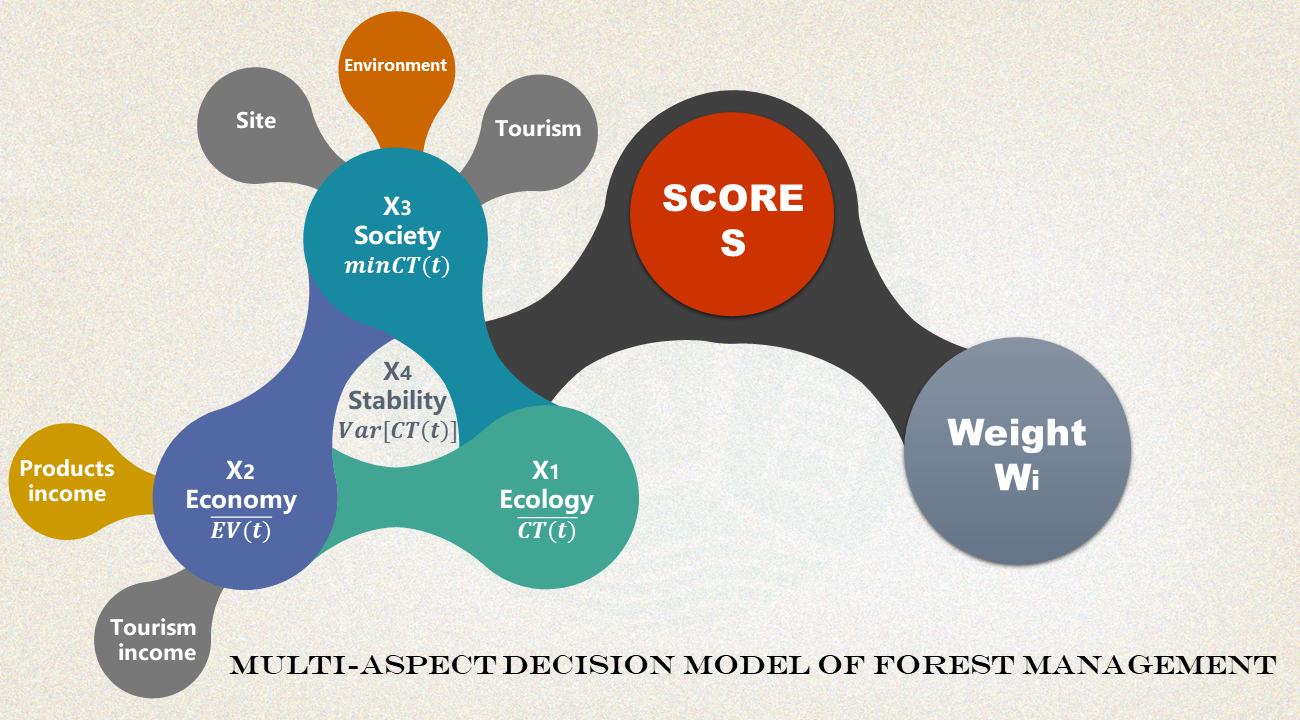
\includegraphics[width=15cm]{figs/multi_model.png}
    \caption{Multi-aspect Decision Model of Forest Management.}
    \label{fig:my_label}
\end{figure}

Based on the definition of forest value\cite{multi_system}, this paper establishes indicators from three traditional dimensions of ecology, society and economy to reflect the comprehensive value of forest based on certain principles, and introduces sustainability variables as references for forest development potential. Finally, the level of ecological, economic and social development of forest system was classified and comprehensively evaluated by entropy weight method. According to the evaluation results of specific forests, the model can provide suggestions for forest management.

The Multi-aspect Decision Model of Forest Management can be summarized in in Figure 3.

\subsection{Evaluation dimensions of forest value}

\subsubsection{Ecological value}
"Canopy density" is considered as a classic index reflecting the ecological value of a forest, which can be used to measure the thickness of a forest. However, the forest data directly reflecting canopy density is difficult to obtain in reality. Through correlation analysis, we can conclude that canopy density is positively correlated with leaf biomass, so variables directly related to biomass can be used as proxy variables.

In the carbon sequestration model, we have concluded that the amount of biological carbon sequestration $CT(t)$is proportional to the biomass, so it can reflect the growth degree of the forest. The greater the biomass, the more mature the forest and the higher its ecological value. Therefore, we derive the following formula to quantitatively calculate forest ecological value.

Considering the long duration of the ecological effect of the forest, we take the average value of carbon sequestration for 100 years as the ecological indicator.

$$
x_1=\overline{CT(t)}
$$


\subsubsection{Economic value}
From the perspective of benefit measurement and ecological compensation, forest economic value is often used as the economic benefit of forest, that is, the monetary expression of forest value in the commodity society. In the process of maintaining the biological characteristics of the forest, the forest products or ecological environment generated in the forest ecosystem and its influence range can be used by people. The monetary expression in the commodity economy is the value of forest economic benefits, which is also called the total economic value of the forest.
%计算过程%

The calculation process of economic value of forest products is as follows:

Sawn-wood       :   $Pr_1$=2300 yuan/cubic meter

Pulp-wood       :   $Pr_2$=5300 yuan/cubic meter

Slash           :   $Pr_3$=900 yuan/ton

$$EV(t)=\sum_{i}H_i(t)\times(\alpha_iPr_{1}+\beta_i Pr_{2}+\gamma_iPr_{3})$$

Finally, take the 100-year average of returns as an economic indicator.

$$x_2=\overline{EV(t)}$$

In the article, the economic value of forest ecosystems was not included in the evaluation of the economic value of forests for the following reasons.

\begin{itemize}
    \item The economic value of forest ecological environment is usually reflected as tourism resources. The development of forest tourism is usually influenced by cultural factors and local socio-economic development, while the change of ecological environment caused by forest management strategy has no significant impact on local socio-economic development.
    \item The marginal returns to the state of forest ecosystems are low. The high level of forest ecology has a small impact on economic returns. The economic benefits of ecological environment can basically only be qualitative but not quantitative.
\end{itemize}

Based on the above reasons, this part of the economic income is included in the social value evaluation dimension of the forest in the model rather than the economic value dimension.

\subsubsection{Social value}

Forest site selection, forest ecology, and the degree of tourism development are important influencing factors and reference indicators of the social value of forests.

In the perspective of forest ecology, we choose the minimum value of biomass as the variable. Forest biomass directly reflects the ecological condition and resource affluence of the forest, which can be regarded as the guaranteed part of the forest available for ecotourism and affects the social value of the forest.

The individual effects of forest site selection and degree of tourism development are significant, and the particular forest site location may play a decisive influence on forest management measures. For example, some forests serve as ecological reserves and are largely free of economic activity. For special cases a separate analysis of the forest site is required.

For conventional forest land, the discussion of forest site location and the degree of tourism development is not significant, and the model discards these two factors for the sake of simplifying the model.

$$
x_3=\min CT(t)
$$

Compared with the hierarchical analysis and fuzzy integrated judgment methods commonly used in social value evaluation, the choice of measurable biomass indicators to quantify the social value of forests can eliminate the subjectivity in value judgment. It is also more direct and objective in data acquisition, which enhances the universality of the model.

\subsubsection{Stability}

As the concept of green development is put forward, the evaluation of forest value should not be limited to the present ecological, economic and social value. In fact, ecological sustainability, economic sustainability and social sustainability are all important components of the evaluation of each dimension.

We need to integrate sustainability principles into forest management measures in order to grasp the potential and potential problems of sustainable development of forests and achieve the desired ecological, economic and social goals.

The stability of forest ecological condition directly reflects the sustainability of forest. We used the statistical variance of carbon sequestration to measure forest sustainability.

$$
x_4=\frac{\sum_{t=1}^{100}(CT(t)-\overline{CT})^2}{100-1}
$$




\subsection{Comprehensive evaluation process of multidimensional value}

The model has addressed the economic, social, ecological and sustainability dimensions of forest values respectively. In order to carry out comprehensive evaluation, we need to homogenize the indicators of each dimension, and give the comprehensive score of forest through entropy weight method, so as to evaluate and guide forest management measures. 

For each index, the values of $n$under different schemes are obtained and scaled to the range of [0,1].

$$
norx_{ij}=\frac{\max x-x}{\max x-\min x}
$$

Calculate the information entropy of each index $E_i$

$$
Y_{ij}=\frac{norx_{ij}}{\sum_{j=1}^n norx_{ij}}
$$
$$
E_i=-\frac{1}{\ln n}\sum_{j=1}^{n}Y_{ij}\ln Y_{ij}
$$

Find out the weight of each indicator $W_i$

$$
W_i=\frac{1-E_i}{4-\sum E_i}
$$

The final score $S$ of the management scheme is calculated as follows.

$$
S=\sum_{i=1}^4 W_i\times x_i'
$$

%待补充
